\documentclass[10pt,a4paper]{report}
\usepackage{graphicx}
\usepackage{siunitx}
\usepackage{caption}
\usepackage{subcaption}
\usepackage{booktabs}

\title{Report Electrical Characterization}
\author{Paul Saß}
\date{November 2026}

\begin{document}


\chapter{Diode Characterization}

\section{Introduction}

For this part of the practical we want to observe the behavior of a p-n junction. For that we consider two diodes, one small and one large, under light and no light. Both devices have a contact on the top of the wafer with which we close the circuit. The other end of the circuit is on the bottom of the wafer which then leads to our SMU. \\
From the measurement with no Voltage we obtain that our cable has a leakage of $\SI{4}{\nano \A}$ which is negledgeble considering the current amplitudes used in the mesurements.



\section{Diodes under light}

First we observe both Diodes under light. For this setup, we leave the wafers exposed to the room light and the light from the microscope. 




\begin{figure}[h!]
        \centering
        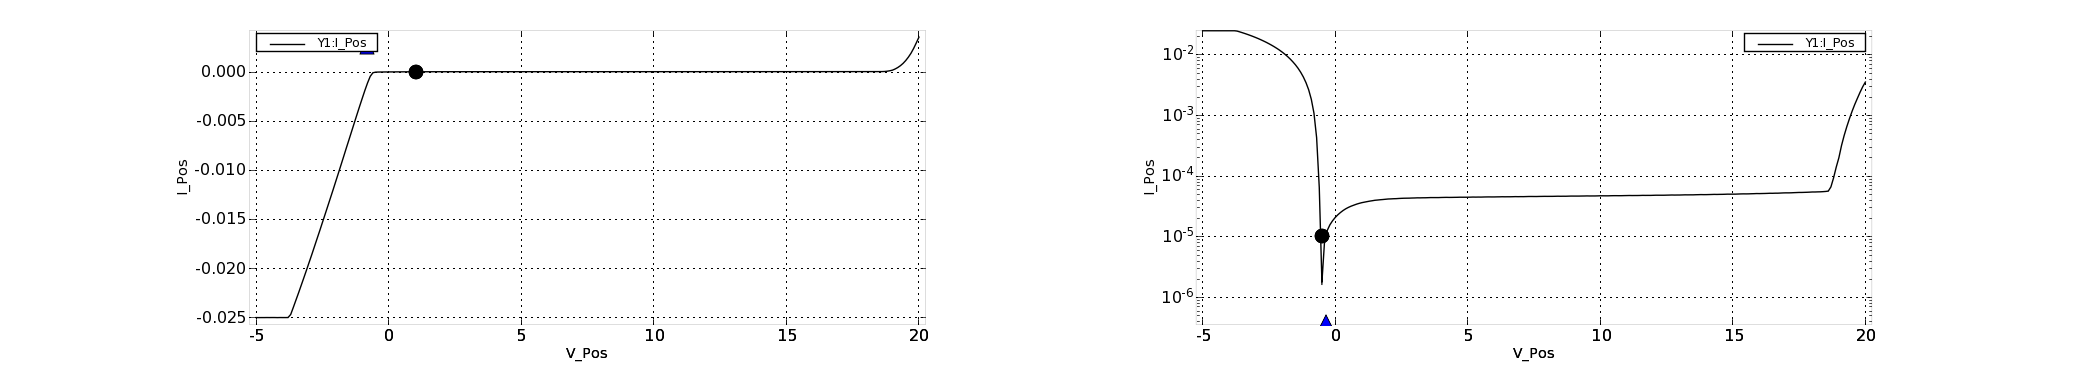
\includegraphics[width=\textwidth]{assets/task2.2.1_small_light 2.png}
        \caption{Small diode}\label{fig:small_light}
\end{figure}
\begin{figure}[h!]
        \centering
        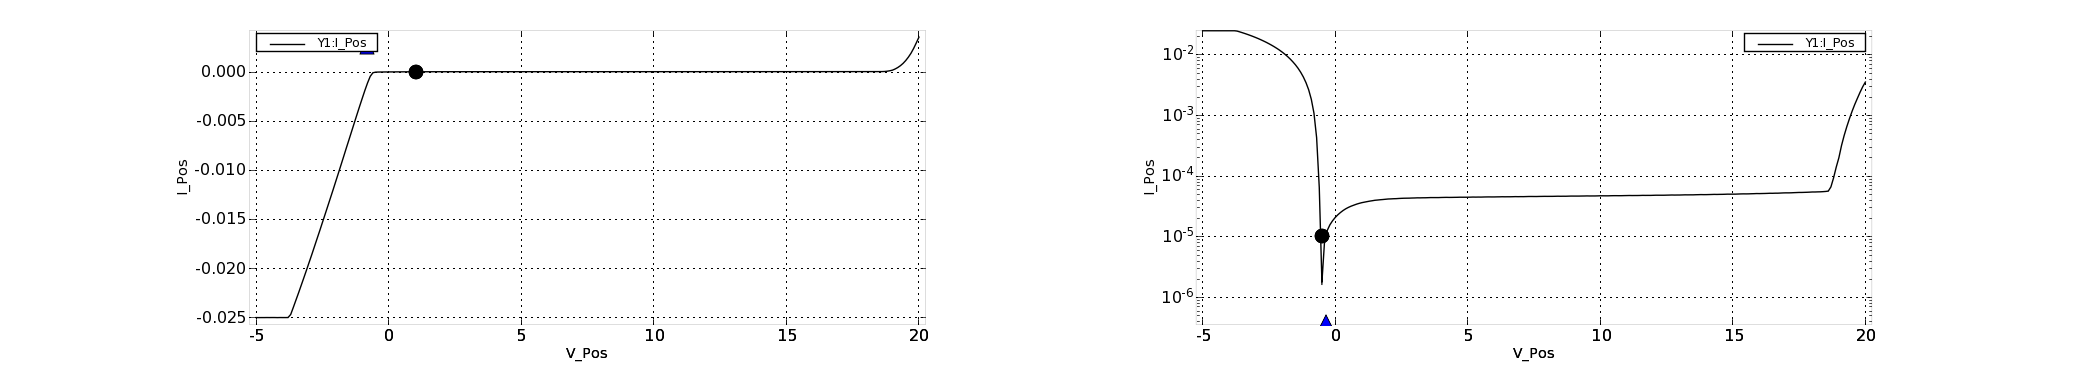
\includegraphics[width=\textwidth]{assets/task2.2.1_small_light 2.png}
        \caption{Large diode}\label{fig:large_light}
\end{figure}

\section{Diodes without light}

\section{Comparison}
\begin{table}[h!]
        \centering
        \begin{tabular}{lcccc}
                \toprule
                Diode & $V_\mathrm{th}$ [V] & $V_a$ [V] & $I(1\,\mathrm{V})$ [$\mu$A] & $I(10\,\mathrm{V})$ [$\mu$A] \\
                \midrule
                Small Light & $-0{,}5$ & $1{,}87$ & $47{,}60$ & $36{,}61$ \\
                Small       & $-0{,}4$ & $1{,}88$ & $3{,}01$  & $3{,}87$  \\
                Large Light & $-0{,}6$ & $1{,}86$ & $51{,}14$ & $55{,}46$ \\
                Large       & $-0{,}5$ & $1{,}87$ & $3{,}93$  & $4{,}31$  \\
                \bottomrule
        \end{tabular}
\end{table}


So what we observe

\section{Calculation of the $n$ factor}
\[
  S =  - \frac{\ln(1.00434e-5) - \ln(8.526250e-7)}{(-0.5) +0.1} \approx \SI {46,446}{ \frac{1}{\V}}
\]
\[
  V_{\text{thermal}} = \frac{k_B T }{q} \approx \SI{25,7}{ \milli \V} = \SI {0,0257} {\V}
\]

\[
  n = \frac {1} {(S \cdot V_\text{thermal})} = 0.838
\]
\section{C-V Characteristic}
\end{document}

